
% Misunderstandings
\begin{frame}{Haller \& Krauss, 2002}

 An independent means t-test results in ($t = 2.7, p = 0.01$). Which of the following are true?
	\begin{itemize}
		\item You have absolutely disproved the null hypothesis.
		\item You have found the probability of the null hypothesis being true.
		\item You have absolutely proved your experimental hypothesis.
		\item You can deduce the probability of the experimental hypothesis being true.
		\item You know, if you decide to reject the null hypothesis, the probability that 	
			  you are making the wrong decision.
		\item You have a reliable experimental finding in the sense that if, 
			  hypothetically, the experiment were repeated a great number of times, you 
			  would obtain a significant result on 99\% of occasions.
	\end{itemize}
\end{frame}
\begin{frame}

\begin{center}
	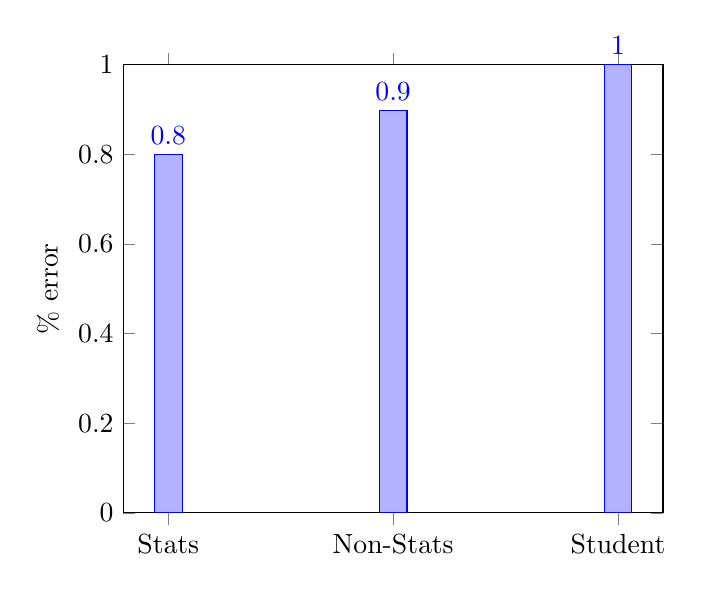
\begin{tikzpicture}
		\begin{axis}[
			ymin=0, ymax = 1,
    			ybar,
    			ylabel={\% error},
    			symbolic x coords={Stats,Non-Stats,Student},
    			xtick=data,
    			nodes near coords,
    			nodes near coords align={vertical},
    			]
			\addplot coordinates {(Stats,.8) (Non-Stats,.897) (Student,1)};
		\end{axis}
	\end{tikzpicture}
\end{center}
\end{frame}
\begin{frame}
Similar:
	\begin{description}
		\item[Oakes (1986)] 97\% Error rate
		\item[Falk and Greenbaum (1995)] 87\% Error rate
	\end{description}
\end{frame}

% The p-value
\begin{frame}{Hypothesis Testing}
	\begin{itemize}
		\pause
		\item Let $X$ be a random sample of size $n$ from a distribution with 
			  finite mean $\mu$ and variance $\sigma^2$. Then (by central limit theorem)
			 \[\bar{X} \xrightarrow{d} \mathrm{N}\left (\mu, \frac{\sigma^2}{n}\right )\]
		\pause
		\item So, if the true mean $\mu$ is zero, then $\bar{X}$ is (approximately) 
			  normally distributed with mean $0$ and standard deviation 
			  $\frac{\sigma}{\sqrt{n}}$.
		\pause
		\item If this is unlikely, then "reject the null".
	\end{itemize}
\end{frame}

\begin{frame}{The p-value is uninteresting}
Setup:
	\begin{itemize}
		\item Police force in a city of 1,000,000 people with 100 criminals
		\item Lie detector with 99\% accuracy
		\item $H_0$: Person is innocent
	\end{itemize}
Experiment:
	\begin{itemize}
		\item Test one person and find guilty.
		\item p-value?
		\pause
		\begin{itemize}
			\item 1\% false positive rate, so $p = 0.01$.
		\end{itemize}
		\pause
		\item Probability that person is actually guilty?
		\pause
		\begin{align*} 
			P(H_1|D) &= \frac{P(D|H_1)P(H_1)}{P(D)} \\
					 &= \frac{0.99 \cdot 0.0001}
					   		 {0.99 \cdot 0.0001 + 0.01 \cdot 0.9999} \\
					 &\approx 0.001
		\end{align*}
	\end{itemize}
\end{frame}

\begin{frame}{The Case for Bayes}
	\begin{itemize}
		\item Gives us what we want: The probability that a hypothesis is true.
		\item Allows us to specify more complex/realistic models.
		\item Allows us to incorporate prior information/research.
	\end{itemize}
\end{frame}
